\documentclass[NET,english,beameralt]{tumbeamer}
% \usepackage[options]{hyperref}
\usepackage{listings}
\documentclass[NET,english,beameralt]{tumbeamer}
\usepackage[options]{minted}
\usepackage[options]{hyperref}
\documentclass[NET,english,beameralt]{tumbeamer}
\usepackage[options]{minted}
\usepackage[options]{hyperref}
\documentclass[NET,english,beameralt]{tumbeamer}
\usepackage[options]{minted}
\usepackage[options]{hyperref}
\input{include/slides}
\beamerdefaultoverlayspecification{<+->}

\begin{document}

\begin{frame}{Agenda}
    \begin{itemize}[<.->]
        \item Starlink 101
        \item trying to understand routing decisions
        \item visualize visible satellites
        \item exploring the GRPC api
    \end{itemize}
\end{frame}

\begin{frame}{Starlink 101}
\begin{figure}
    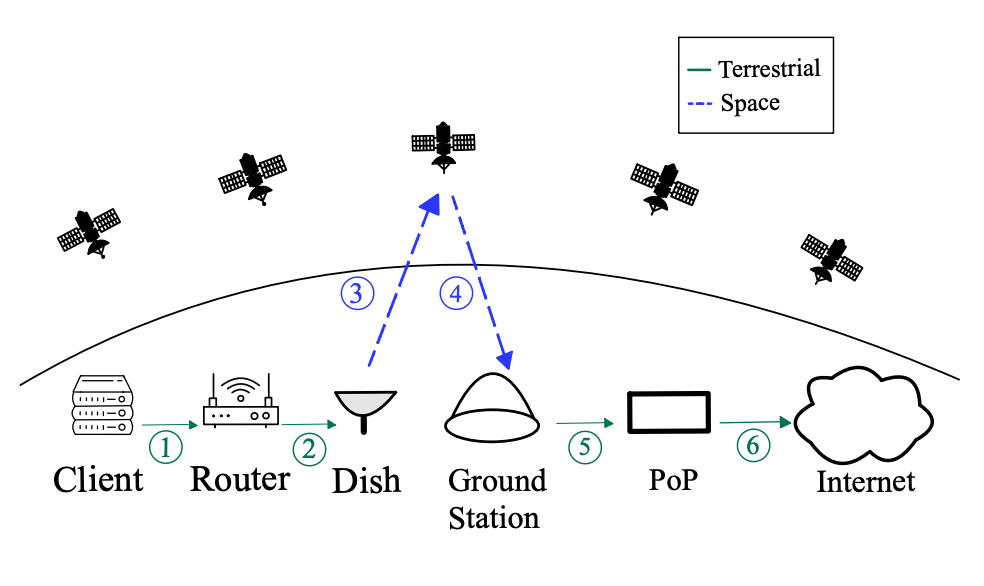
\includegraphics[width=0.75\textwidth]{pics/starlink-101.png}
    \caption[short]{Basic Starlink working (ignoring ISL), from \cite{izhikevich2023democratizing}}
\end{figure}
\end{frame}

\begin{frame}{Understanding routing decisions}
\begin{itemize}
    \item got ip address blocks from major cloud providers (aws,azure,oracle), as we know their position \footnote[]{the fact we know the position doesn't really mean a traceroute to a certain address is really a traceroute to that geographic area}
    \item chose 5 geographically sparse targets around the globe (for aws: ap-northeast-2, us-east-1, ap-south-1, sa-east-1, me-south-1 )
    \item tracerouted the targets over several days 
\end{itemize}
\end{frame}

\begin{frame}{Understanding routing decisions}
\begin{figure}
    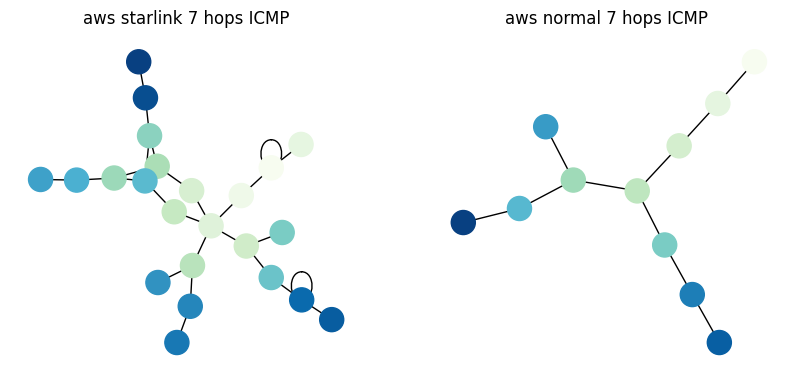
\includegraphics[width=0.75\textwidth]{pics/aws_7_icmp.png}
    \caption[short]{First 7 hops of traceroutes to 5 AWS datacenters using ICMP}
\end{figure}
\end{frame}

\begin{frame}{Understanding routing decisions}
\begin{figure}
    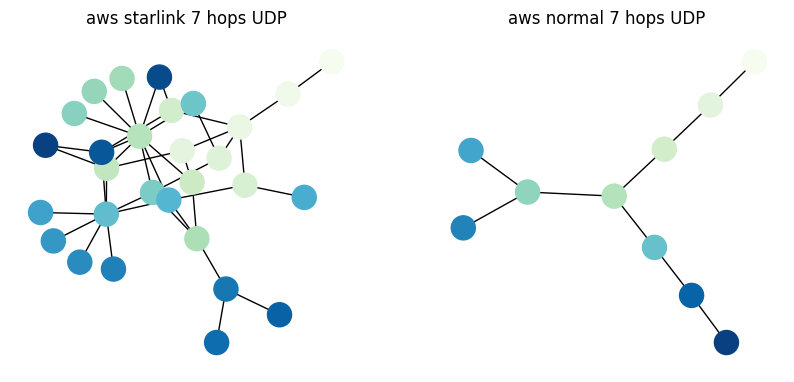
\includegraphics[width=0.75\textwidth]{pics/aws_7_udp.png}
    \caption[short]{First 7 hops of traceroutes to 5 AWS datacenters using UDP}
\end{figure}
\end{frame}

\begin{frame}{Understanding routing decisions}
\begin{figure}
    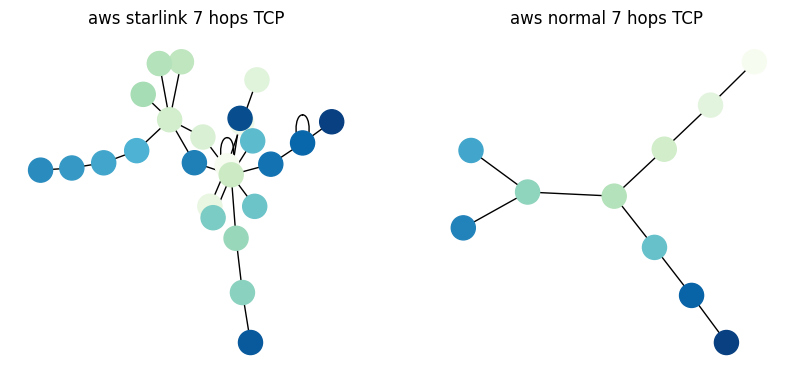
\includegraphics[width=0.75\textwidth]{pics/aws_7_tcp.png}
    \caption[short]{First 7 hops of traceroutes to 5 AWS datacenters using TCP}
\end{figure}
\end{frame}

\begin{frame}{measuring RTT changes when applying stress iperf}
\begin{figure}
    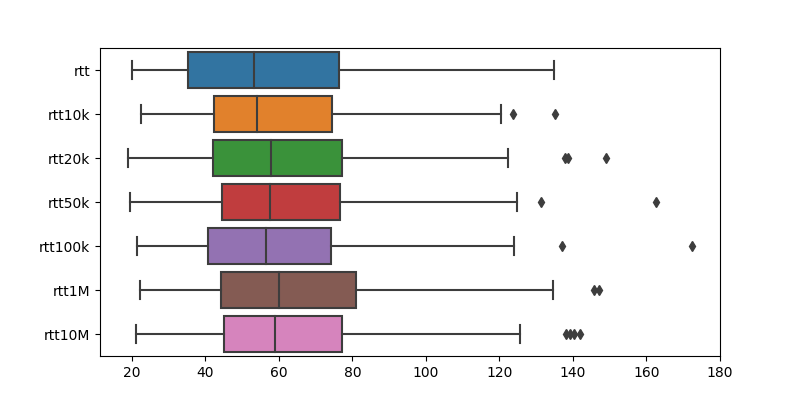
\includegraphics[width=1\textwidth]{pics/rtt-iperf-stress.png}
    \caption[short]{measuring RTT changes when applying stress iperf}
\end{figure}
\end{frame}

\begin{frame}{Visualize visible satellites}
\begin{itemize}
    \item from \href{celestrak.org}{celestrak.org} we can download a list of Starlink's satellites TLEs
    \item A two-line element set (TLE) is a data format encoding a list of orbital elements of an Earth-orbiting object for a given point in time, the epoch. Using a suitable prediction formula, the state (position and velocity) at any point in the past or future can be estimated to some accuracy. (from wikipedia.org)
\end{itemize}
\end{frame}

\begin{frame}[fragile]{\texttt{common.calculate\_visible\_satellites}}
\begin{minted}[fontsize=\small]{python3}
def calculate_visible_satellites(...):
    # ...
    satellites = load.tle_file(stations_url)
    observer = Topos(observer_latitude, observer_longitude, observer_elevation)
    t = load.timescale().now()

    # Calculate satellite positions
    positions = [(sat, (sat - observer).at(t)) for sat in satellites]
    
    # Filter visible satellites
    visible_satellites = []
    for sat, position in positions:
        alt, az, distance = position.altaz()
        # Satellite is above the horizon
        if alt.degrees > 0 and distance.km < distance_km:
            visible_satellites.append((sat, alt, az))

    return visible_satellites
\end{minted}
\end{frame}

\begin{frame}{count of visible satellites across time}
\begin{figure}
    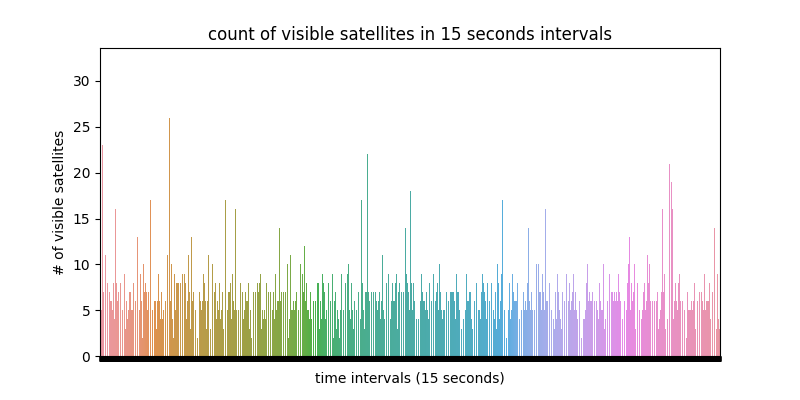
\includegraphics[width=1\textwidth]{pics/count_visible_satellites.png}
    \caption[short]{count of visible satellites across time}
\end{figure}
\end{frame}

\begin{frame}{visualizing patterns in visible satellites}
\begin{figure}
    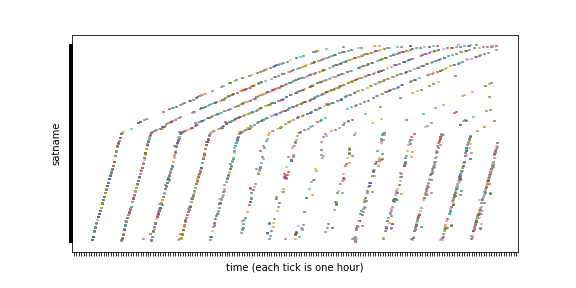
\includegraphics[width=1\textwidth]{pics/visualizing-how-long-satellites-are-visible-for.png}
    \caption[short]{visualizing patterns in visible satellites}
\end{figure}
\end{frame}

\begin{frame}{the gRPC api}
\begin{itemize}
    \item the dish exposes a gRPC api with server reflection, "runtime construction of requests without having stub information precompiled into the client." \footnote{\href{https://github.com/grpc/grpc/blob/master/doc/server-reflection.md}{https://github.com/grpc/grpc/blob/master/doc/server-reflection.md}}
    \item 55 "methods" are available, most of them don't work, we have 2 categories of errors: \texttt{Uninmplemented}, \texttt{PermissionDenied} and a couple of some other specific errors 
    \item working methods: \texttt{reboot}, \texttt{get\_status}, \texttt{start\_dish\_self\_test}, \texttt{get\_history}, \texttt{get\_device\_info}, \texttt{dish\_power\_save}, \texttt{dish\_get\_config}, \texttt{get\_obstruction\_map}
    \item to see all methods: \href{https://hedgedoc.net.in.tum.de/N7nACD1OSk2x2e7biPHJTA}{https://hedgedoc.net.in.tum.de/N7nACD1OSk2x2e7biPHJTA}
\end{itemize}
\end{frame}

\begin{frame}{next actions}
\begin{itemize}
    \item investigate satellite handovers following the method described in \cite{izhikevich2023democratizing} (we have a script working)
    \item try to correlate satellite handovers with sudden drops in bandwidth
    \item sneak peak: \href{https://youtu.be/PjfMPr20suw}{https://youtu.be/PjfMPr20suw}
\end{itemize}
\end{frame}

\section{Bibliography}
\begin{frame}[allowframebreaks]
    \bibliographystyle{abbrv}
    \setbeamertemplate{bibliography item}[text]
    \footnotesize
    \bibliography{lit}
\end{frame}

\end{document}

\beamerdefaultoverlayspecification{<+->}

\begin{document}

\begin{frame}{Agenda}
    \begin{itemize}[<.->]
        \item Starlink 101
        \item trying to understand routing decisions
        \item visualize visible satellites
        \item exploring the GRPC api
    \end{itemize}
\end{frame}

\begin{frame}{Starlink 101}
\begin{figure}
    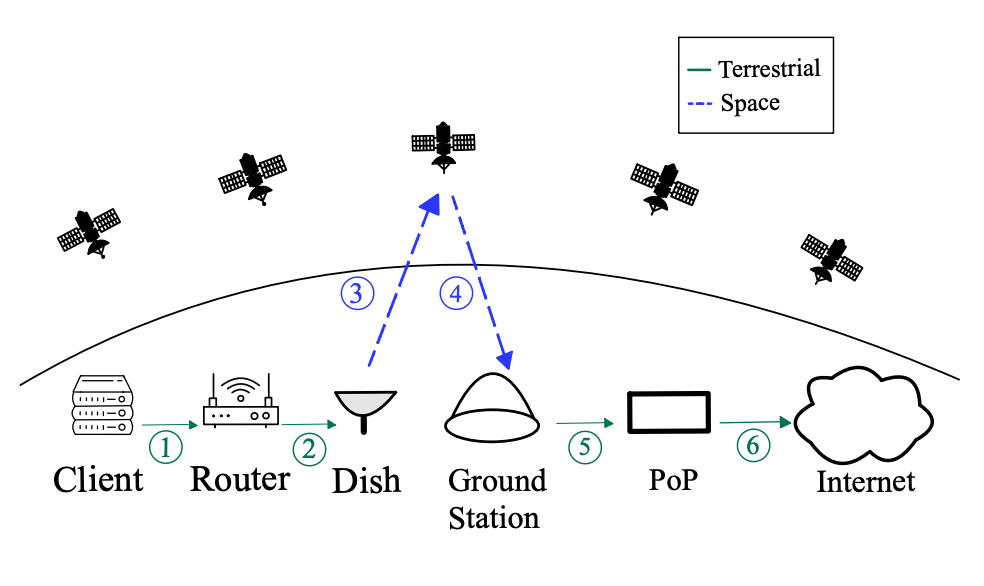
\includegraphics[width=0.75\textwidth]{pics/starlink-101.png}
    \caption[short]{Basic Starlink working (ignoring ISL), from \cite{izhikevich2023democratizing}}
\end{figure}
\end{frame}

\begin{frame}{Understanding routing decisions}
\begin{itemize}
    \item got ip address blocks from major cloud providers (aws,azure,oracle), as we know their position \footnote[]{the fact we know the position doesn't really mean a traceroute to a certain address is really a traceroute to that geographic area}
    \item chose 5 geographically sparse targets around the globe (for aws: ap-northeast-2, us-east-1, ap-south-1, sa-east-1, me-south-1 )
    \item tracerouted the targets over several days 
\end{itemize}
\end{frame}

\begin{frame}{Understanding routing decisions}
\begin{figure}
    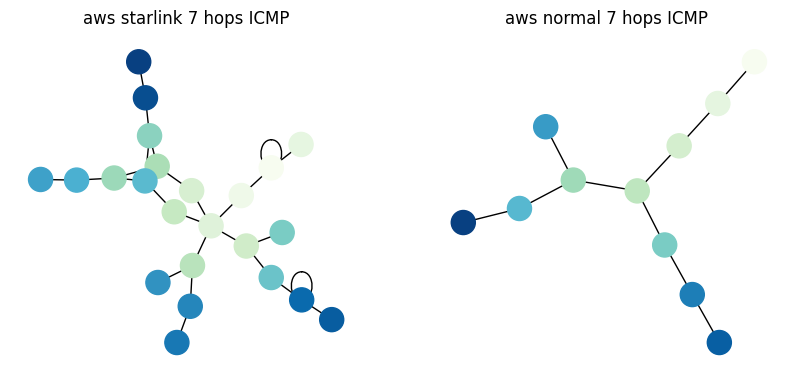
\includegraphics[width=0.75\textwidth]{pics/aws_7_icmp.png}
    \caption[short]{First 7 hops of traceroutes to 5 AWS datacenters using ICMP}
\end{figure}
\end{frame}

\begin{frame}{Understanding routing decisions}
\begin{figure}
    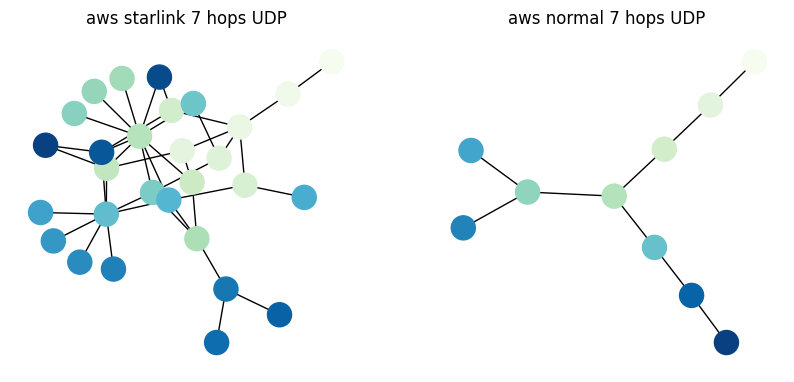
\includegraphics[width=0.75\textwidth]{pics/aws_7_udp.png}
    \caption[short]{First 7 hops of traceroutes to 5 AWS datacenters using UDP}
\end{figure}
\end{frame}

\begin{frame}{Understanding routing decisions}
\begin{figure}
    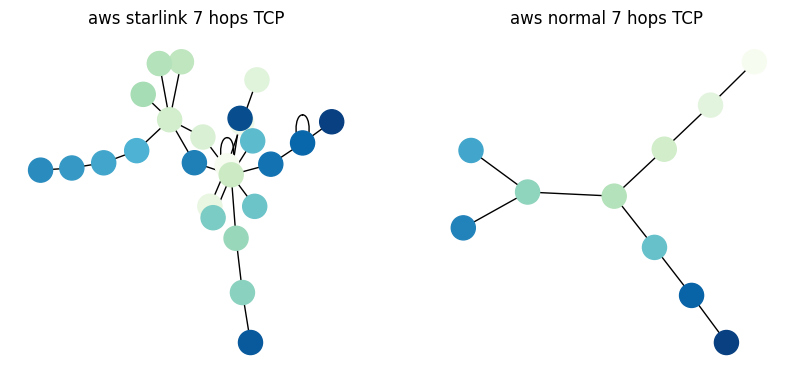
\includegraphics[width=0.75\textwidth]{pics/aws_7_tcp.png}
    \caption[short]{First 7 hops of traceroutes to 5 AWS datacenters using TCP}
\end{figure}
\end{frame}

\begin{frame}{measuring RTT changes when applying stress iperf}
\begin{figure}
    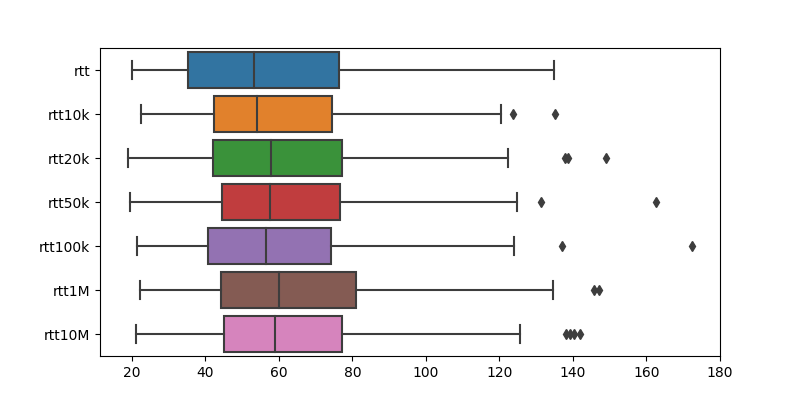
\includegraphics[width=1\textwidth]{pics/rtt-iperf-stress.png}
    \caption[short]{measuring RTT changes when applying stress iperf}
\end{figure}
\end{frame}

\begin{frame}{Visualize visible satellites}
\begin{itemize}
    \item from \href{celestrak.org}{celestrak.org} we can download a list of Starlink's satellites TLEs
    \item A two-line element set (TLE) is a data format encoding a list of orbital elements of an Earth-orbiting object for a given point in time, the epoch. Using a suitable prediction formula, the state (position and velocity) at any point in the past or future can be estimated to some accuracy. (from wikipedia.org)
\end{itemize}
\end{frame}

\begin{frame}[fragile]{\texttt{common.calculate\_visible\_satellites}}
\begin{minted}[fontsize=\small]{python3}
def calculate_visible_satellites(...):
    # ...
    satellites = load.tle_file(stations_url)
    observer = Topos(observer_latitude, observer_longitude, observer_elevation)
    t = load.timescale().now()

    # Calculate satellite positions
    positions = [(sat, (sat - observer).at(t)) for sat in satellites]
    
    # Filter visible satellites
    visible_satellites = []
    for sat, position in positions:
        alt, az, distance = position.altaz()
        # Satellite is above the horizon
        if alt.degrees > 0 and distance.km < distance_km:
            visible_satellites.append((sat, alt, az))

    return visible_satellites
\end{minted}
\end{frame}

\begin{frame}{count of visible satellites across time}
\begin{figure}
    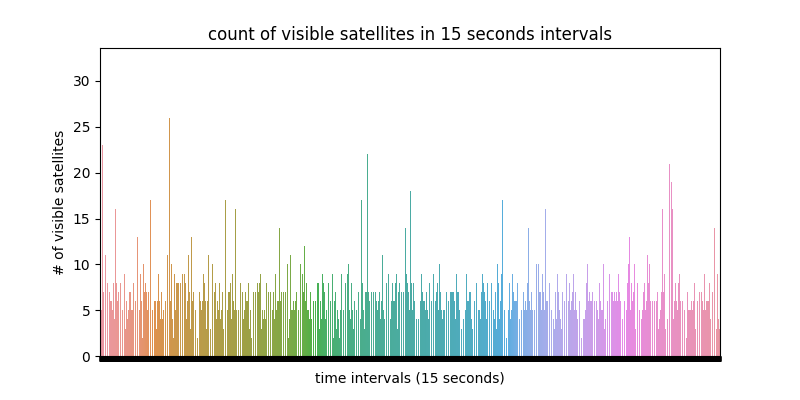
\includegraphics[width=1\textwidth]{pics/count_visible_satellites.png}
    \caption[short]{count of visible satellites across time}
\end{figure}
\end{frame}

\begin{frame}{visualizing patterns in visible satellites}
\begin{figure}
    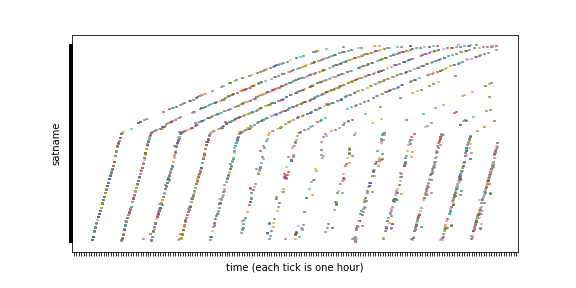
\includegraphics[width=1\textwidth]{pics/visualizing-how-long-satellites-are-visible-for.png}
    \caption[short]{visualizing patterns in visible satellites}
\end{figure}
\end{frame}

\begin{frame}{the gRPC api}
\begin{itemize}
    \item the dish exposes a gRPC api with server reflection, "runtime construction of requests without having stub information precompiled into the client." \footnote{\href{https://github.com/grpc/grpc/blob/master/doc/server-reflection.md}{https://github.com/grpc/grpc/blob/master/doc/server-reflection.md}}
    \item 55 "methods" are available, most of them don't work, we have 2 categories of errors: \texttt{Uninmplemented}, \texttt{PermissionDenied} and a couple of some other specific errors 
    \item working methods: \texttt{reboot}, \texttt{get\_status}, \texttt{start\_dish\_self\_test}, \texttt{get\_history}, \texttt{get\_device\_info}, \texttt{dish\_power\_save}, \texttt{dish\_get\_config}, \texttt{get\_obstruction\_map}
    \item to see all methods: \href{https://hedgedoc.net.in.tum.de/N7nACD1OSk2x2e7biPHJTA}{https://hedgedoc.net.in.tum.de/N7nACD1OSk2x2e7biPHJTA}
\end{itemize}
\end{frame}

\begin{frame}{next actions}
\begin{itemize}
    \item investigate satellite handovers following the method described in \cite{izhikevich2023democratizing} (we have a script working)
    \item try to correlate satellite handovers with sudden drops in bandwidth
    \item sneak peak: \href{https://youtu.be/PjfMPr20suw}{https://youtu.be/PjfMPr20suw}
\end{itemize}
\end{frame}

\section{Bibliography}
\begin{frame}[allowframebreaks]
    \bibliographystyle{abbrv}
    \setbeamertemplate{bibliography item}[text]
    \footnotesize
    \bibliography{lit}
\end{frame}

\end{document}

\beamerdefaultoverlayspecification{<+->}

\begin{document}

\begin{frame}{Agenda}
    \begin{itemize}[<.->]
        \item Starlink 101
        \item trying to understand routing decisions
        \item visualize visible satellites
        \item exploring the GRPC api
    \end{itemize}
\end{frame}

\begin{frame}{Starlink 101}
\begin{figure}
    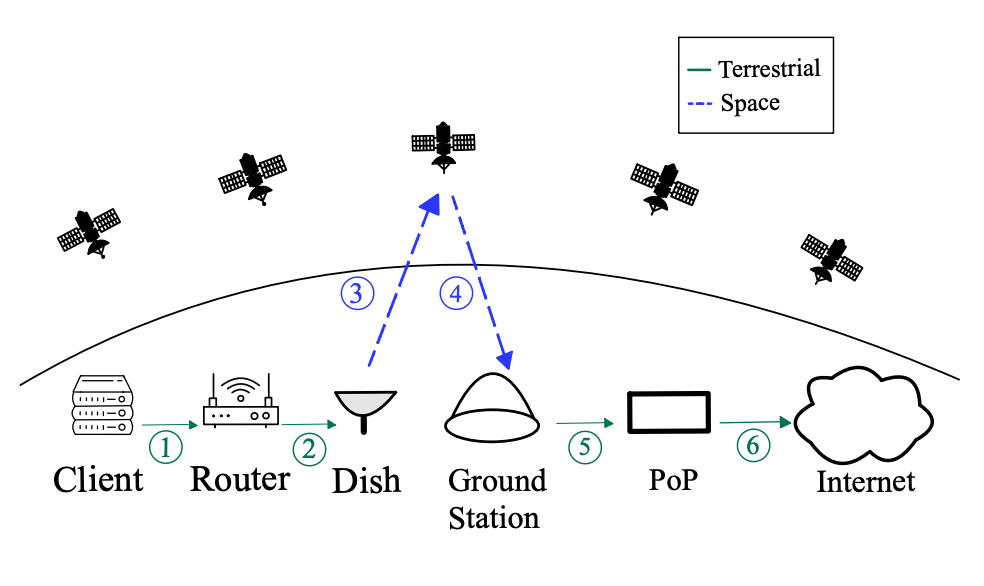
\includegraphics[width=0.75\textwidth]{pics/starlink-101.png}
    \caption[short]{Basic Starlink working (ignoring ISL), from \cite{izhikevich2023democratizing}}
\end{figure}
\end{frame}

\begin{frame}{Understanding routing decisions}
\begin{itemize}
    \item got ip address blocks from major cloud providers (aws,azure,oracle), as we know their position \footnote[]{the fact we know the position doesn't really mean a traceroute to a certain address is really a traceroute to that geographic area}
    \item chose 5 geographically sparse targets around the globe (for aws: ap-northeast-2, us-east-1, ap-south-1, sa-east-1, me-south-1 )
    \item tracerouted the targets over several days 
\end{itemize}
\end{frame}

\begin{frame}{Understanding routing decisions}
\begin{figure}
    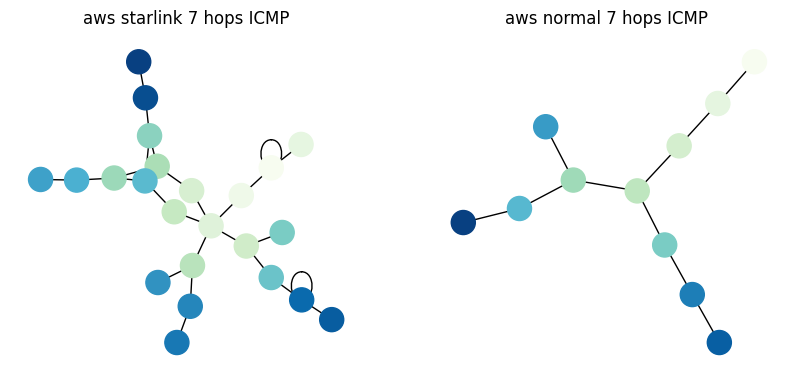
\includegraphics[width=0.75\textwidth]{pics/aws_7_icmp.png}
    \caption[short]{First 7 hops of traceroutes to 5 AWS datacenters using ICMP}
\end{figure}
\end{frame}

\begin{frame}{Understanding routing decisions}
\begin{figure}
    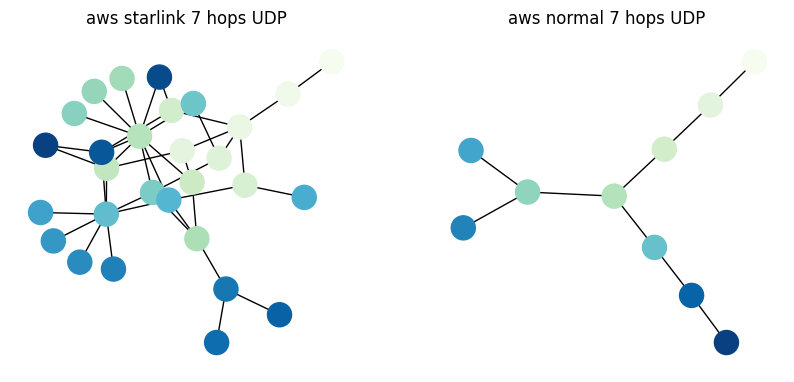
\includegraphics[width=0.75\textwidth]{pics/aws_7_udp.png}
    \caption[short]{First 7 hops of traceroutes to 5 AWS datacenters using UDP}
\end{figure}
\end{frame}

\begin{frame}{Understanding routing decisions}
\begin{figure}
    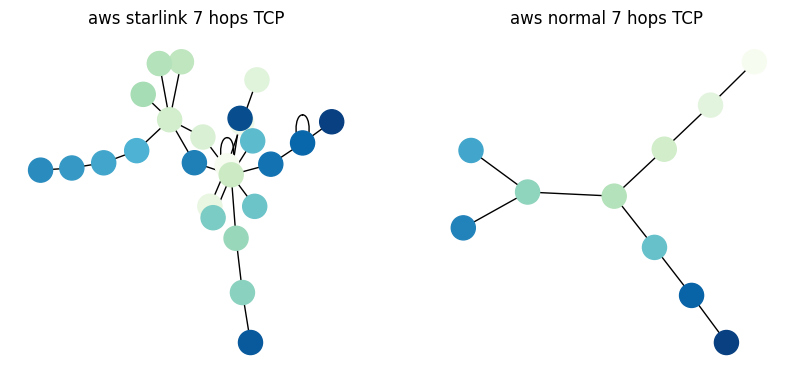
\includegraphics[width=0.75\textwidth]{pics/aws_7_tcp.png}
    \caption[short]{First 7 hops of traceroutes to 5 AWS datacenters using TCP}
\end{figure}
\end{frame}

\begin{frame}{measuring RTT changes when applying stress iperf}
\begin{figure}
    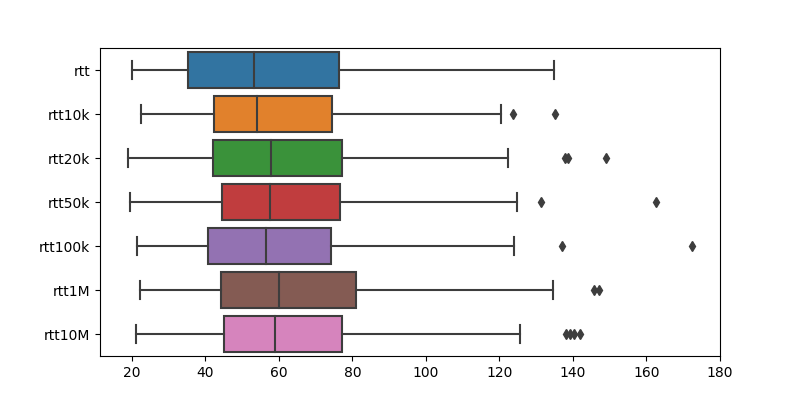
\includegraphics[width=1\textwidth]{pics/rtt-iperf-stress.png}
    \caption[short]{measuring RTT changes when applying stress iperf}
\end{figure}
\end{frame}

\begin{frame}{Visualize visible satellites}
\begin{itemize}
    \item from \href{celestrak.org}{celestrak.org} we can download a list of Starlink's satellites TLEs
    \item A two-line element set (TLE) is a data format encoding a list of orbital elements of an Earth-orbiting object for a given point in time, the epoch. Using a suitable prediction formula, the state (position and velocity) at any point in the past or future can be estimated to some accuracy. (from wikipedia.org)
\end{itemize}
\end{frame}

\begin{frame}[fragile]{\texttt{common.calculate\_visible\_satellites}}
\begin{minted}[fontsize=\small]{python3}
def calculate_visible_satellites(...):
    # ...
    satellites = load.tle_file(stations_url)
    observer = Topos(observer_latitude, observer_longitude, observer_elevation)
    t = load.timescale().now()

    # Calculate satellite positions
    positions = [(sat, (sat - observer).at(t)) for sat in satellites]
    
    # Filter visible satellites
    visible_satellites = []
    for sat, position in positions:
        alt, az, distance = position.altaz()
        # Satellite is above the horizon
        if alt.degrees > 0 and distance.km < distance_km:
            visible_satellites.append((sat, alt, az))

    return visible_satellites
\end{minted}
\end{frame}

\begin{frame}{count of visible satellites across time}
\begin{figure}
    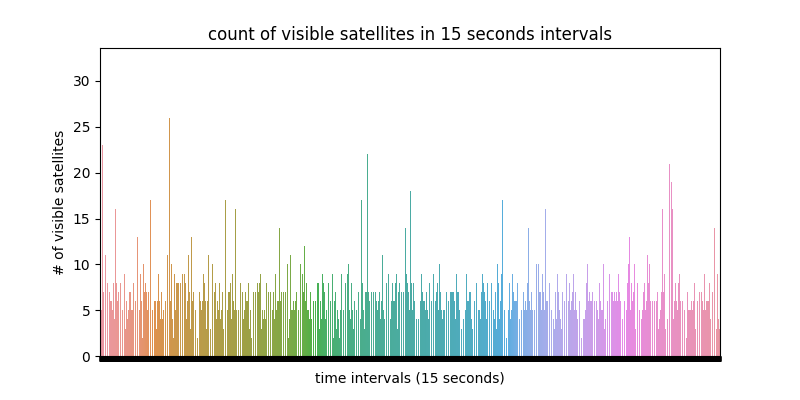
\includegraphics[width=1\textwidth]{pics/count_visible_satellites.png}
    \caption[short]{count of visible satellites across time}
\end{figure}
\end{frame}

\begin{frame}{visualizing patterns in visible satellites}
\begin{figure}
    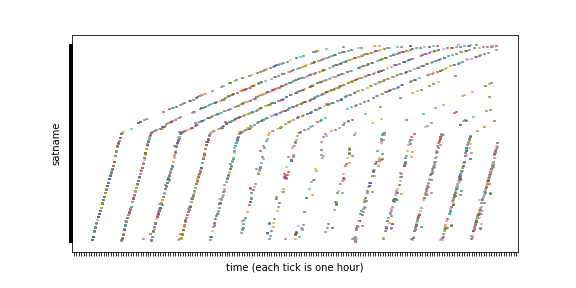
\includegraphics[width=1\textwidth]{pics/visualizing-how-long-satellites-are-visible-for.png}
    \caption[short]{visualizing patterns in visible satellites}
\end{figure}
\end{frame}

\begin{frame}{the gRPC api}
\begin{itemize}
    \item the dish exposes a gRPC api with server reflection, "runtime construction of requests without having stub information precompiled into the client." \footnote{\href{https://github.com/grpc/grpc/blob/master/doc/server-reflection.md}{https://github.com/grpc/grpc/blob/master/doc/server-reflection.md}}
    \item 55 "methods" are available, most of them don't work, we have 2 categories of errors: \texttt{Uninmplemented}, \texttt{PermissionDenied} and a couple of some other specific errors 
    \item working methods: \texttt{reboot}, \texttt{get\_status}, \texttt{start\_dish\_self\_test}, \texttt{get\_history}, \texttt{get\_device\_info}, \texttt{dish\_power\_save}, \texttt{dish\_get\_config}, \texttt{get\_obstruction\_map}
    \item to see all methods: \href{https://hedgedoc.net.in.tum.de/N7nACD1OSk2x2e7biPHJTA}{https://hedgedoc.net.in.tum.de/N7nACD1OSk2x2e7biPHJTA}
\end{itemize}
\end{frame}

\begin{frame}{next actions}
\begin{itemize}
    \item investigate satellite handovers following the method described in \cite{izhikevich2023democratizing} (we have a script working)
    \item try to correlate satellite handovers with sudden drops in bandwidth
    \item sneak peak: \href{https://youtu.be/PjfMPr20suw}{https://youtu.be/PjfMPr20suw}
\end{itemize}
\end{frame}

\section{Bibliography}
\begin{frame}[allowframebreaks]
    \bibliographystyle{abbrv}
    \setbeamertemplate{bibliography item}[text]
    \footnotesize
    \bibliography{lit}
\end{frame}

\end{document}


\begin{document}

\begin{frame}{What is Starlink?}
	\begin{itemize}
		\item Starlink Low Earth Orbiting (LEO) Satellite Constellation
		\item Brings Internet connection to remote areas 
		\item More than 4000 Satellites with plans to launch more
		\item End users have a Dish that connect to satellites in sight
		\item Performance is higher compared to Geostationary Satellites (GEOSAT) based connections
		\item Average Latency is ~35ms and Download Bandwidth is >100 MBps
	\end{itemize}
\end{frame}

\begin{frame}{Starlink 101}
	\begin{figure}
    	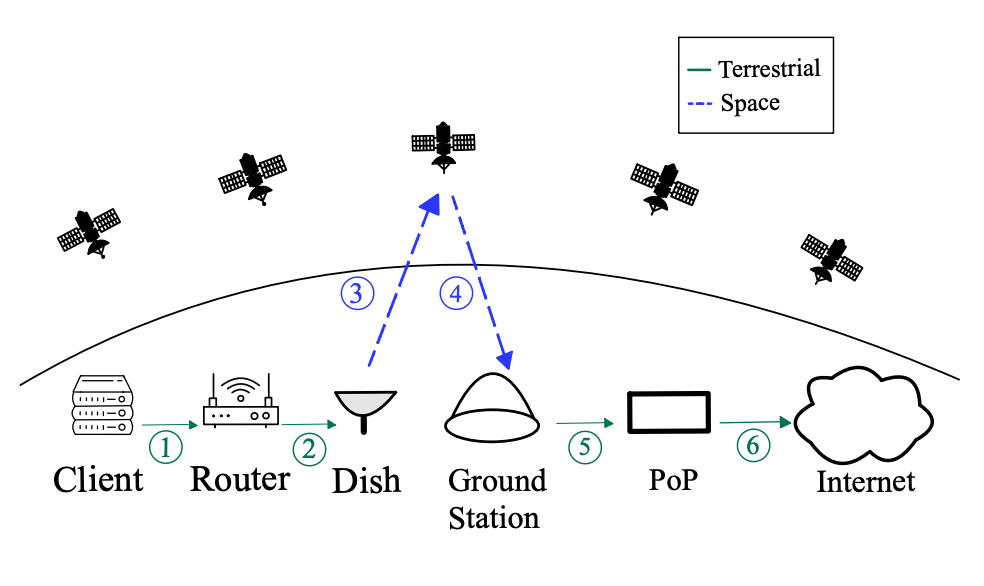
\includegraphics[width=0.75\textwidth]{pics/starlink-101.png}
    	\caption{Starlink in a nutshell (ignoring ISL), from \cite{izhikevich2023democratizing}}
	\end{figure}
\end{frame}

\begin{frame}{Our Dish}
	\begin{figure}
    	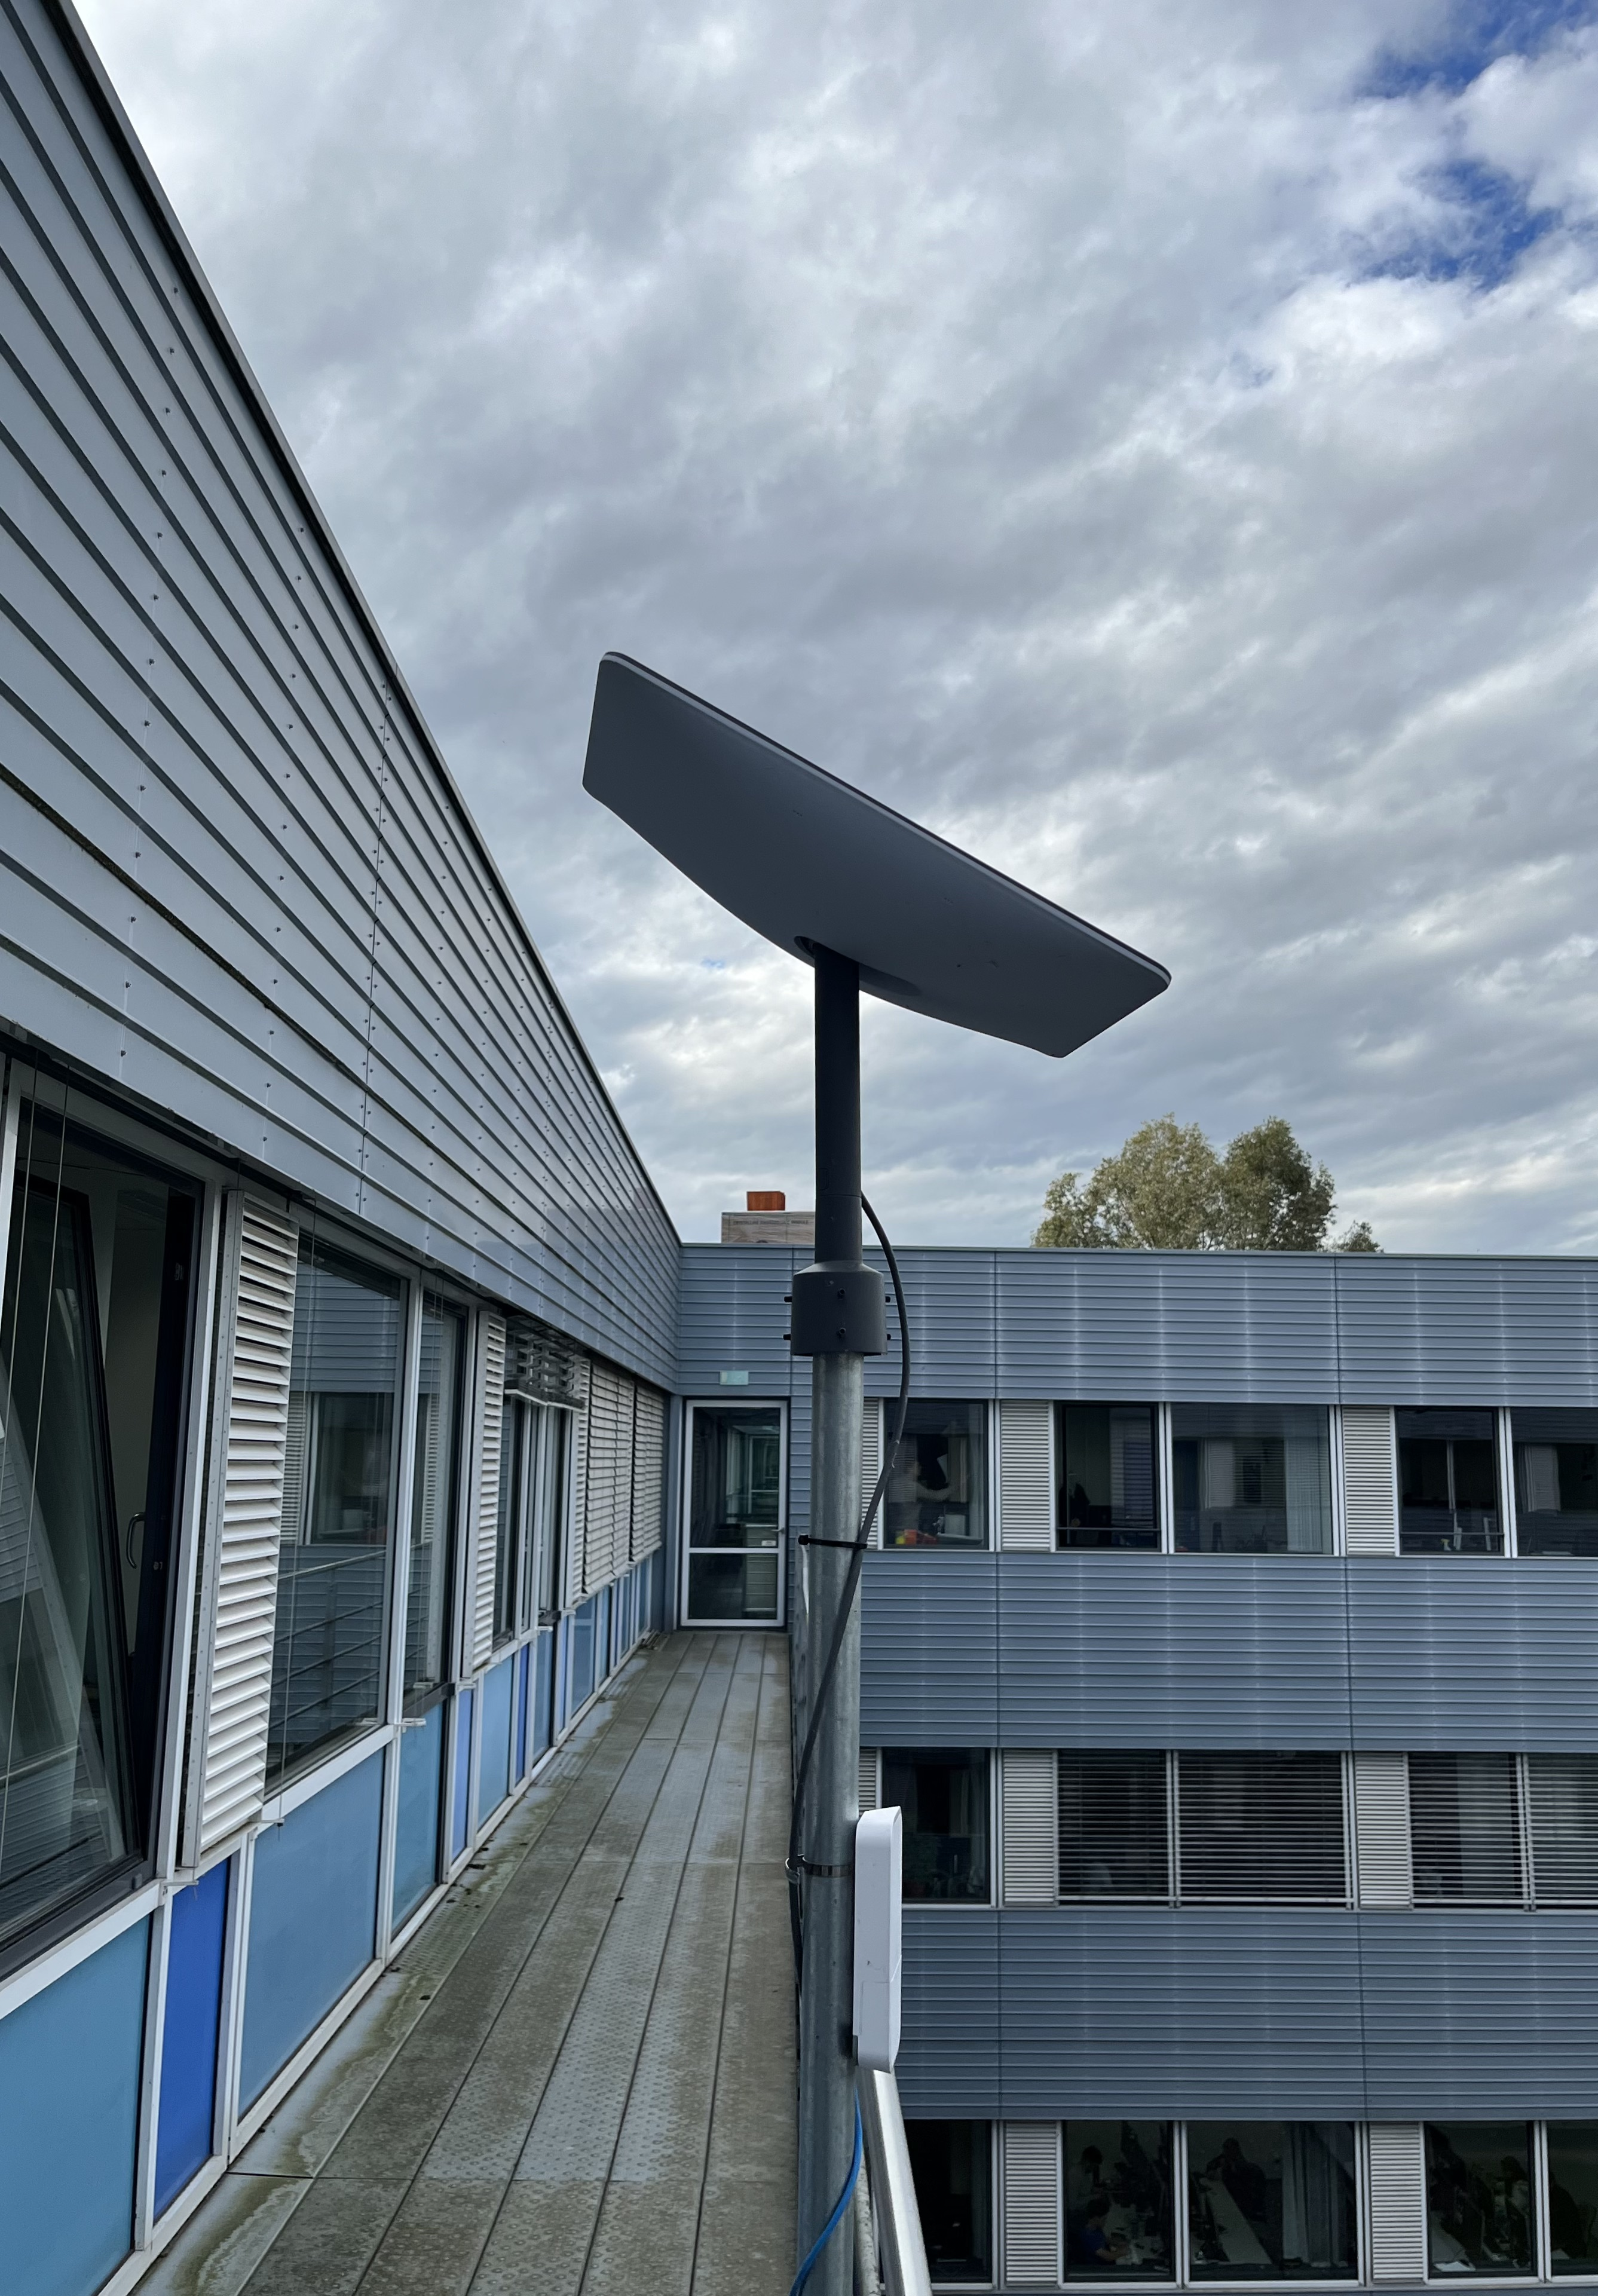
\includegraphics[width=0.3\textwidth]{pics/dish.jpeg}
    	\caption{Our Starlink Dish}
	\end{figure}
\end{frame}

\begin{frame}{Our Work}
	\begin{itemize}
		\item Understanding Routing Decisions
		\item Visualize Visible Satellites and patterns in their apperance
		\item Physical Layer Influcences on Performance
		\item Documenting gRPC API
		\item Retrieval of Obstruction Maps
		\item Satellite Handovers detection based on Obstruction Maps
		\item Correlation between Satellite Handovers and Bandwidth Drops	
	\end{itemize}
\end{frame}

\begin{frame}{Understanding Routing Decisions}
	\begin{itemize}
		\item retrieved ip address blocks from major cloud providers (aws,azure,oracle), as we know their position
			\footnote{the fact we know the position doesn't really the last hop will be exactly in that area (little infomation around
            what happens inside datacenters), but it is a good enough approximation}
		\item chose 5 geographically sparse targets around the globe, i.e for aws:
            \begin{itemize}
                \item \texttt{ap-northeast-2} Asia Pacific (Seoul)
                \item \texttt{us-east-1} US East (N. Virginia)
                \item \texttt{ap-south-1} Asia Pacific (Mumbai)
                \item \texttt{sa-east-1} South America (São Paulo)
                \item \texttt{me-south-1} Middle East (Bahrain)
            \end{itemize}
    	\item tracerouted the targets over several days 
	\end{itemize}
\end{frame}

\begin{frame}{Understanding Routing Decisions}
	\begin{figure}
    	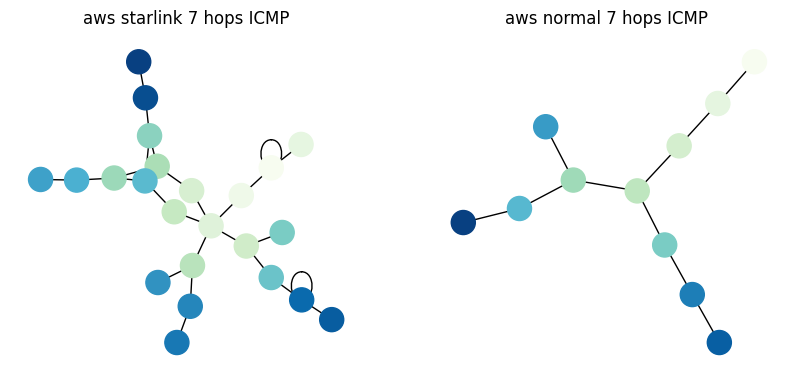
\includegraphics[width=0.75\textwidth]{pics/aws_7_icmp.png}
    	\caption[short]{First 7 hops of traceroutes to 5 AWS datacenters using ICMP}
	\end{figure}
\end{frame}

\begin{frame}{Visualize Visible Satellites}
	\begin{itemize}
    	\item from \href{celestrak.org}{celestrak.org} we can download a list of Starlink's satellites TLEs
		\item A two-line element set (TLE) is a data format encoding a list of orbital elements of an Earth-orbiting
			object for a given point in time, the epoch. 
		\item Using a suitable prediction formula, the state (position and velocity) at any point in the past or future
			can be estimated to some accuracy. (from wikipedia.org)
		\item wrote a Python script to calculate visible
		satellites\footnote{\url{https://gitlab.lrz.de/netintum/teaching/tumi8-theses/idp-castellotti/-/blob/main/common.py?ref_type=heads\#L132}}
        \item Gathered information about satellites position and proceeded to visualize how often we see a satellite
    \end{itemize}
\end{frame}

\begin{frame}{Visualizing Patterns in Visible Satellites}
    \begin{figure}
        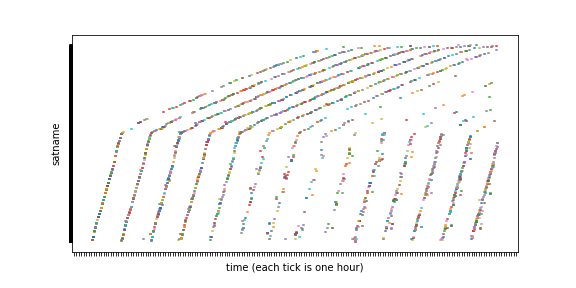
\includegraphics[width=1\textwidth]{pics/patterns-in-satellite-appearances.png}
    \end{figure}
\end{frame}

\begin{frame}{Pysical Layer Influences on Performance}
	\begin{itemize}
		\item sent packets with iPerf to create traffic on the interface
		\item downloded Debian ISOs from 5 different mirrors (neutralize upload speed differences)
	\end{itemize}
    \begin{figure}
        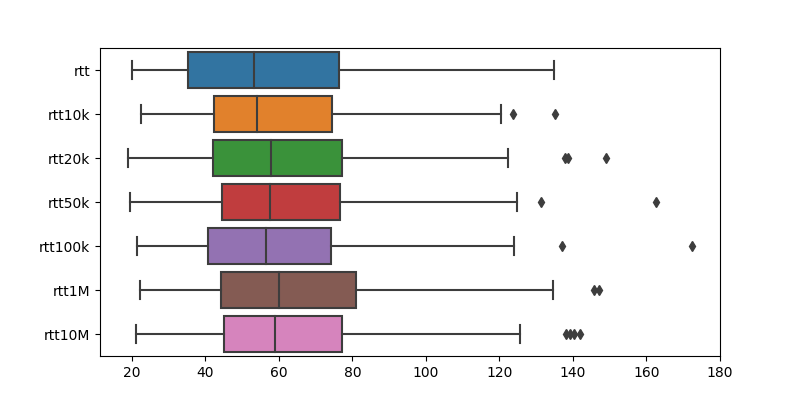
\includegraphics[width=1\textwidth]{pics/rtt-iperf-stress.png}
    \end{figure}
\end{frame}

\begin{frame}{The gRPC api}
    \begin{itemize}
		\item the dish exposes a gRPC api with server reflection, "runtime construction of requests without having stub
        information precompiled into the client."
		\footnote{\url{https://github.com/grpc/grpc/blob/master/doc/server-reflection.md}}
        \item 55 "methods" are available, most of them don't work, we have 2 categories of errors: \texttt{Uninmplemented},
        \texttt{PermissionDenied} and a couple of some other specific errors 
        \item most interesting working methods: 
            \begin{itemize}
                \item \texttt{reboot}
                \item \texttt{get\_status}
                \item \texttt{get\_obstruction\_map}
            \end{itemize}
        \item all methods: \url{https://gist.github.com/rcastellotti/e20630366dfeaeada6cc2680f562f6ac}
    \end{itemize}
\end{frame}


\begin{frame}{the \texttt{dish\_get\_obstruction\_map} Endpoint}
    \begin{itemize}
        \item the \texttt{dish\_get\_obstruction\_map} endpoint seems interesting
        \item an Obstruction Map captures the position where the dish has seen satellites up to that moment
        \item designed to provide a way to report whether the dish position is optimal
        \item following the approach described by Izhikevich et al. \cite{izhikevich2023democratizing} we retrieve maps
        \item rebooting the dish clears the Obstruction Map
        \item polling the endpoint frequently enough allows us to detect satellite handovers
        \item we start by saving maps every second, we then proceed to visualize them
    \end{itemize}
\end{frame}

\begin{frame}[fragile]{Querying the  \texttt{dish\_get\_obstruction\_map} Endpoint }
    \begin{lstlisting}[
        % basicstyle=\footnotesize,
    ]
"apiVersion":"9",
"dishGetObstructionMap":{
    "minElevationDeg":10.0,
    "numCols":123,
    "numRows":123,
    "snr":[-1.0,-1.0,-1.0,-1.0,...,1.0,1.0,-1.0,-1.0]
}
    \end{lstlisting}
\end{frame}

\begin{frame}[fragile]{Visualizing a single Obstruction Map}
    \begin{lstlisting}[
        captionpos=b,
        basicstyle=\small,
    ]
import json
import numpy as np
import matplotlib.pyplot as plt

map = json.load(open("1692089163.json"))
map = map["dishGetObstructionMap"]["snr"]
map = np.array(map).reshape(123, 123) # a 123*123 matrix
plt.imshow(map)
plt.show()
    \end{lstlisting}
\end{frame}

\begin{frame}[fragile]
    \begin{figure}
        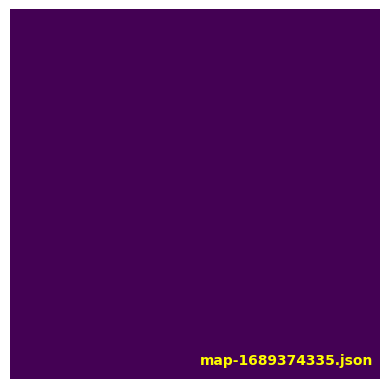
\includegraphics[width=0.4\columnwidth]{pics/map1.png}
    \end{figure}
\end{frame}

\begin{frame}[fragile]
    \begin{figure}
        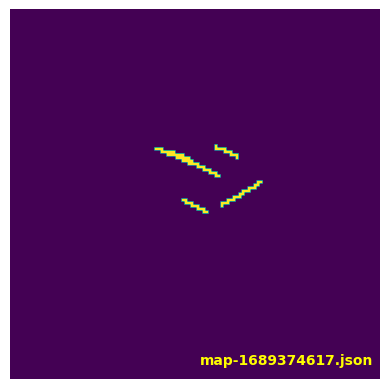
\includegraphics[width=0.4\columnwidth]{pics/map2.png}
    \end{figure}
\end{frame}

\begin{frame}[fragile]
    \begin{figure}
        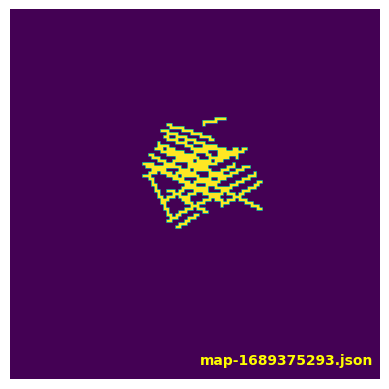
\includegraphics[width=0.4\columnwidth]{pics/map3.png}
    \end{figure}
\end{frame}

\begin{frame}[fragile]
    \begin{figure}
        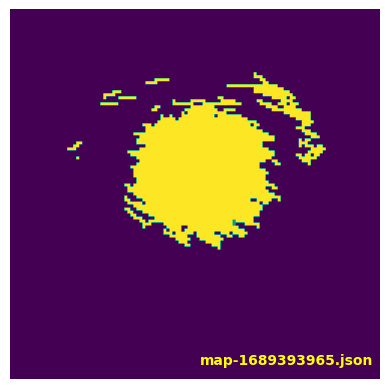
\includegraphics[width=0.4\columnwidth]{pics/map4.png}
    \end{figure}
\end{frame}

\begin{frame}{Detecting Handovers Algoritmically}
    \begin{itemize}
        \item going through visualizations frame by frame is not feasible
        \item interpet obstruction maps as matrices 
        \item "1" means a satellite was seen in that position, "-1" means no satellite was detected
        \item iterate through matrices two by two to detect handovers 
        \item sum matrices
        \item check if "0" value is "near" (inside a 3*3 matrix)
            \begin{itemize}
                \item if it is "near" \emph{no handover was performed}
                \item if it is in complete separate position \emph{an handover must have been performed}
            \end{itemize}
    \end{itemize}
\end{frame}

\begin{frame}{Obstruction Maps as Matrices (No Handover)}
    $\begin{bmatrix}
        -1 & -1 & \color{red}1 &           -1 & -1 \\
        -1 & -1 &           -1 & \color{red}1 & -1 \\
        -1 & -1 &           -1 &           -1 & -1 \\
        -1 & -1 &           -1 &           -1 & -1 \\
        -1 & -1 &           -1 &           -1 & -1 \\ 
        \end{bmatrix}
        +
        \begin{bmatrix}
        -1 & -1 & \color{red}1 &           -1 &           -1 \\
        -1 & -1 &           -1 & \color{red}1 &           -1 \\
        -1 & -1 &           -1 &           -1 & \color{red}1 \\
        -1 & -1 &           -1 &           -1 &           -1 \\
        -1 & -1 &           -1 &           -1 &           -1 \\
        \end{bmatrix}
        =
        \begin{bmatrix}
        -2 & -2 & 2 &  -2 &           -2 \\
        -2 & -2 & -2 &  2 &           -2 \\
        -2 & -2 & -2 & -2 & \color{red}0 \\
        -2 & -2 & -2 & -2 &            -2 \\
        -2 & -2 & -2 & -2 &            -2 \\
    \end{bmatrix}$
\end{frame}

\begin{frame}{Obstruction Maps as Matrices (Handover)}
    $\begin{bmatrix}
        -1 & -1 & \color{red}1 &           -1 & -1 \\
        -1 & -1 &           -1 & \color{red}1 & -1 \\
        -1 & -1 &           -1 &           -1 & -1 \\
        -1 & -1 &           -1 &           -1 & -1 \\
        -1 & -1 &           -1 &           -1 & -1 \\
    \end{bmatrix}
    +
    \begin{bmatrix}
        -1 & -1 & \color{red}1 &           -1 & -1 \\
        -1 & -1 &           -1 & \color{red}1 & -1 \\
        -1 & -1 &           -1 &           -1 & -1 \\
        -1 & -1 &           -1 &           -1 & -1 \\
        1 & -1 &            -1 &           -1 & -1 \\
    \end{bmatrix}
    =
    \begin{bmatrix}
        -2 & -2 & 2 & -2 & -2 \\
        -2 & -2 & -2 & 2 & -2 \\
        -2 & -2 & -2 & -2 & -2 \\
        -2 & -2 & -2 & -2 & -2 \\
        \color{red}0 & -2 & -2 & -2 & -2 \\
    \end{bmatrix}$
\end{frame}

\begin{frame}[fragile]{Correlation between Satellite Handovers and Bandwidth Drops}
    \begin{itemize}
        \item we have an algorithm to detect handovers
        \item we run in parallel 2 scripts
            \begin{itemize}
                \item 1st: retrieves an obstruction map every second
                \item 2nd: gathers Bandwidth data
            \end{itemize} 
        \item we visualize Bandwidth data and satellite handovers 
    \end{itemize}
\end{frame}


\begin{frame}[fragile]{Correlation between Satellite Handovers and Bandwidth Drops}
    \begin{figure}
        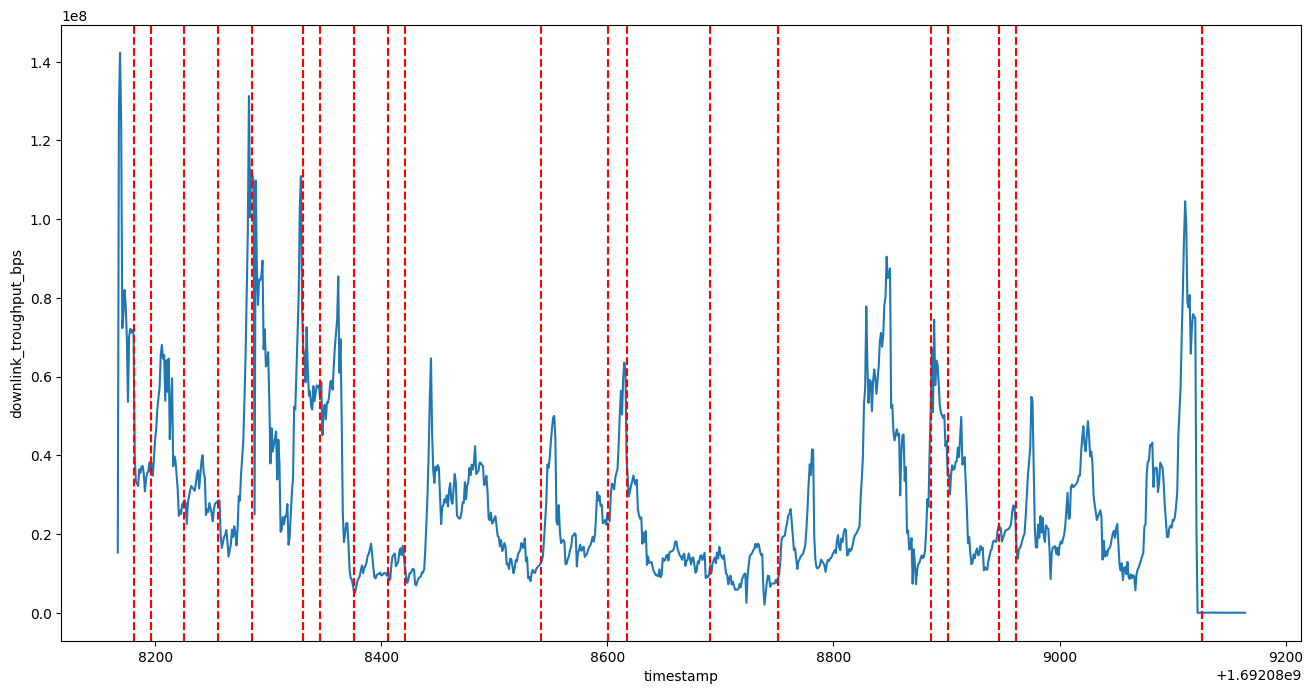
\includegraphics[width=0.8\columnwidth]{pics/correlation_handovers_bw.png}
    \end{figure}
\end{frame}


% slide similar tech
% mention where to find report with all the code
% slide further work
% thanks leander and johannes and carle for preseting starlink during ACN
% sumup all the experiments

\section{Bibliography}
\begin{frame}[allowframebreaks]
    \bibliographystyle{abbrv}
    \setbeamertemplate{bibliography item}[text]
    \footnotesize
    \bibliography{lit}
\end{frame}

\end{document}
